\section{Core Principles of Radar and Sensing}
\label{sec:radar_sensing_fundamentals}

In the previous discussion, we reviewed how a wireless system transmits,
receives, and recovers information bits from the perspective of digital
communication.
Unlike a communication system, whose primary objective is to recover the
information carried by the transmitted signal, a radar or sensing system aims
to obtain state information about targets and the surrounding physical
environment from the echoes generated through the interaction between the
transmitted signal and the environment.

This section does not provide a complete derivation of radar theory.
Instead, it focuses on target detection, parameter estimation, target tracking,
echo formation, performance metrics, and the basic processing flow.
The purpose is to outline the fundamental concepts in radar sensing that are
closely related to subsequent ISAC system modeling and joint design.

\subsection{Radar Sensing Tasks and Echo-Based Parameter Extraction}

\topichead{Basic Tasks of Radar Sensing Systems}

The basic tasks of radar sensing form a hierarchy from target existence
determination to target state characterization.
Target detection determines whether a target exists in the observation region;
parameter estimation obtains quantities such as range, velocity, and angle; and
target tracking describes the evolution of these states over time.

\topichead{Target Detection}
Target detection decides between ``target present'' and ``target absent'' from
the received signal.
It is the prerequisite for parameter estimation and tracking, and it involves a
tradeoff between missed detection and false alarm.

\topichead{Parameter Estimation}
Parameter estimation further characterizes the target state after detection.
Common parameters include range, velocity, and angle, which describe target
position and motion and support later tracking and scene understanding.
\topichead{Target Tracking}
Target tracking continuously updates the target state across multiple
observation instants.
It forms trajectories and supports interpretation of motion trends such as
approaching, moving away, turning, or accelerating.

\topichead{Echo Formation}
Radar echoes result from the interaction among the transmitted signal, the
target, and the propagation environment.
After reflection or scattering, the echo returns with amplitude attenuation,
delay, phase variation, and possible Doppler shift.
These changes carry range, velocity, and angle information, so radar parameter
extraction analyzes how the echo differs from the transmitted signal.

\topichead{Range Estimation}
Range estimation is based on the echo delay relative to the transmitted signal.
A simplified echo model is
\begin{equation}
    r(t)=\alpha s(t-\tau)e^{j2\pi f_D t}+n(t),
    \label{eq:simplified_radar_echo_model}
\end{equation}
where \(s(t)\) denotes the known signal transmitted by the radar,
\(r(t)\) denotes the received echo, \(\alpha\) denotes the amplitude
coefficient caused by propagation attenuation and target reflection properties,
\(\tau\) denotes the propagation delay of the echo relative to the transmitted
signal, \(f_D\) denotes the Doppler shift caused by target motion, and \(n(t)\)
denotes noise.
This model represents the echo as a delayed, attenuated, and frequency-shifted
version of the transmitted signal.

For a monostatic radar, the signal travels from radar to target and back.
As illustrated in Fig.~\ref{fig:range_estimation_monostatic_radar}, a target
at range \(R\) produces a round-trip propagation distance \(2R\).

\begin{figure}[htbp]
    \centering
    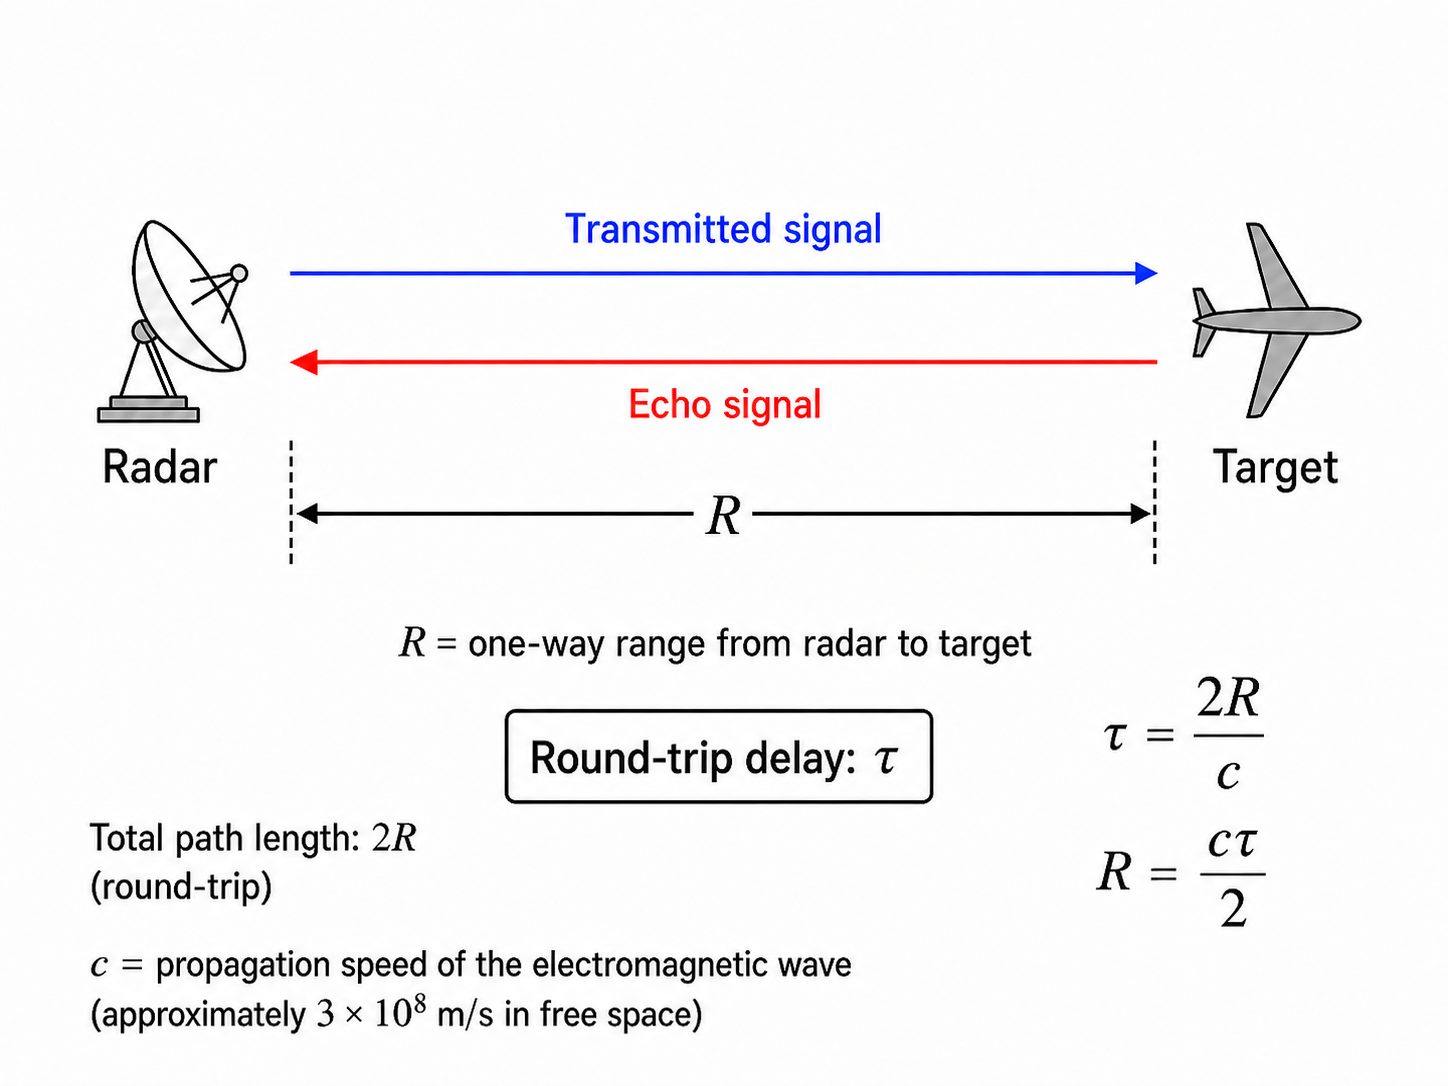
\includegraphics[width=0.62\textwidth]{figures/chapter2/fig_range_estimation.png}
    \caption{Range estimation in a monostatic radar.}
    \label{fig:range_estimation_monostatic_radar}
\end{figure}

If the propagation speed of the electromagnetic wave is \(c\), and the
round-trip propagation delay of the echo is \(\tau\), then the total
propagation distance satisfies
\begin{equation}
    2R=c\tau.
    \label{eq:round_trip_range_delay}
\end{equation}
Thus, the target range can be expressed as
\begin{equation}
    R=\frac{c\tau}{2}.
    \label{eq:radar_range_estimation}
\end{equation}
The factor \(2\) reflects the radar--target--radar round trip.
\topichead{Velocity Estimation}
Velocity estimation is based on the Doppler shift of the echo.
For a moving target, the line-of-sight distance changes with time, producing a
frequency shift related to the radial velocity.
As illustrated in Fig.~\ref{fig:velocity_estimation_monostatic_radar}, this
radial component describes whether the target is approaching or moving away
from the radar.

\begin{figure}[htbp]
    \centering
    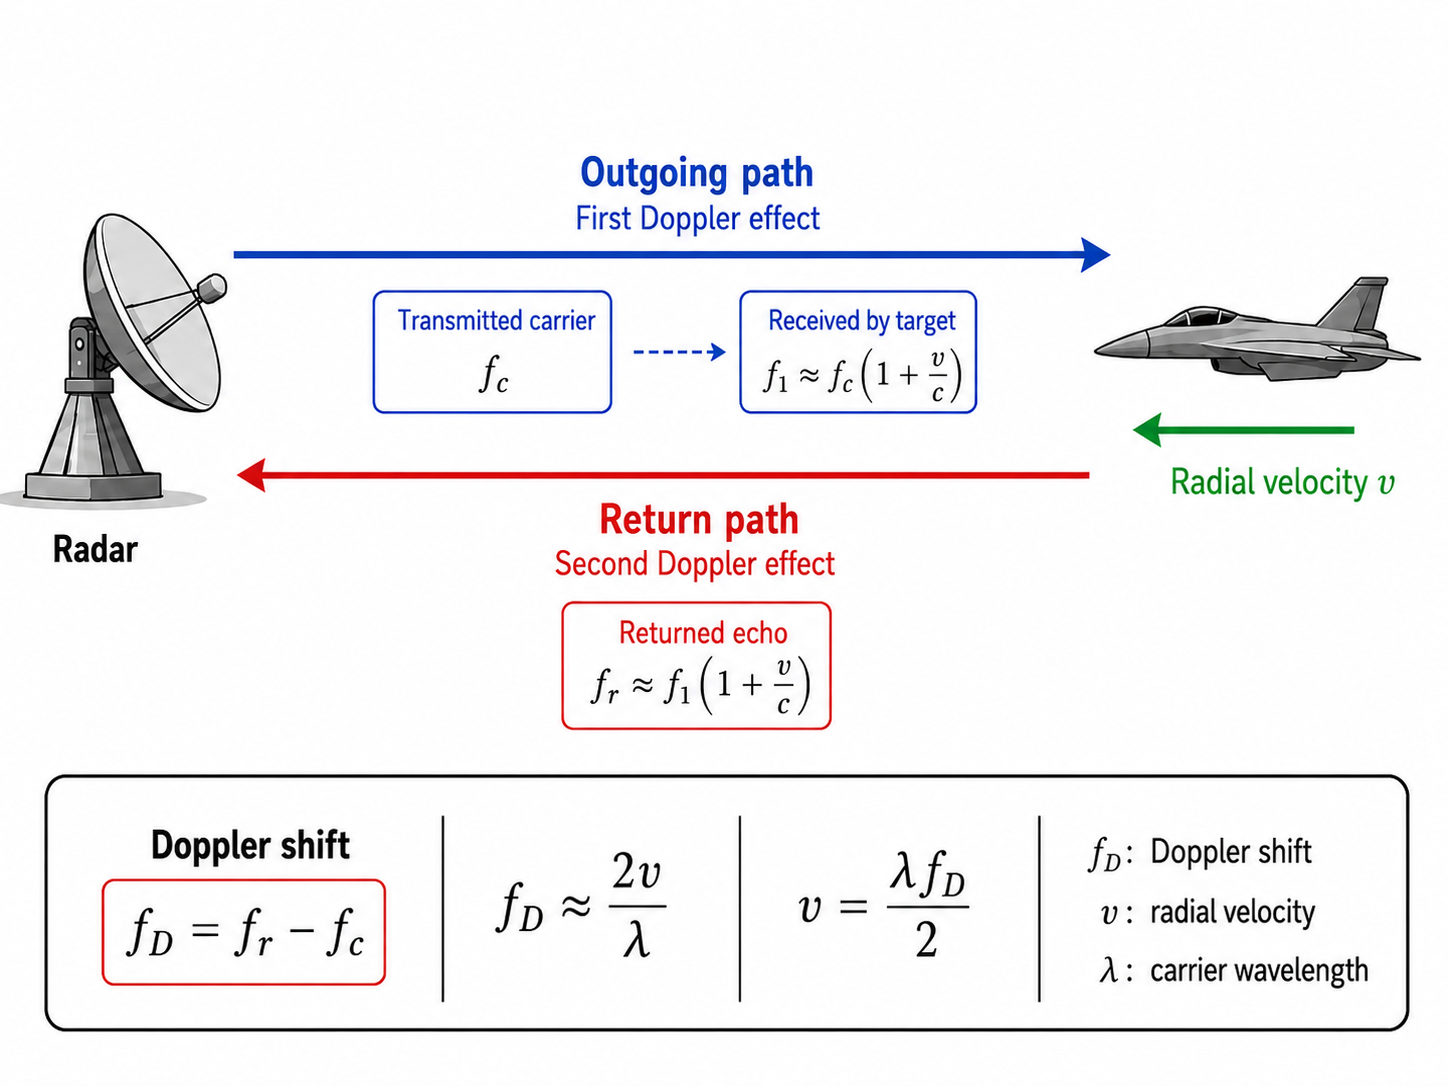
\includegraphics[width=0.62\textwidth]{figures/chapter2/fig_velocity_estimation.png}
    \caption{Velocity estimation in a monostatic radar.}
    \label{fig:velocity_estimation_monostatic_radar}
\end{figure}

For a monostatic radar, target motion affects both the outgoing and return
paths, so the radial velocity \(v\) and Doppler shift \(f_D\) are commonly
related by
\begin{equation}
    f_D=\frac{2v}{\lambda},
    \label{eq:radar_doppler_shift}
\end{equation}
or equivalently,
\begin{equation}
    v=\frac{\lambda f_D}{2},
    \label{eq:radar_velocity_estimation}
\end{equation}
where \(\lambda\) denotes the carrier wavelength.
The factor \(2\) again reflects the two-way propagation.
Approaching and receding targets correspond to Doppler shifts with opposite
signs, while the above equations describe the basic magnitude relationship.

\topichead{Angle Estimation}
Angle estimation relies on spatial phase differences across an antenna array.
A single antenna may provide delay and Doppler information, but direction of
arrival generally requires multiple spatial samples.
For an array, different propagation path lengths to different elements produce
phase differences related to the echo direction.

Consider a uniform linear array as an example.
Let \(d\) denote the spacing between adjacent antenna elements, \(\lambda\)
denote the carrier wavelength, and \(\theta\) denote the angle between the
incident direction of the target echo and the array broadside direction.
As illustrated in Fig.~\ref{fig:angle_estimation_antenna_array}, the path
difference between adjacent antenna elements can be expressed as
\begin{equation}
    \Delta l = d\sin\theta.
    \label{eq:array_path_difference}
\end{equation}

\begin{figure}[htbp]
    \centering
    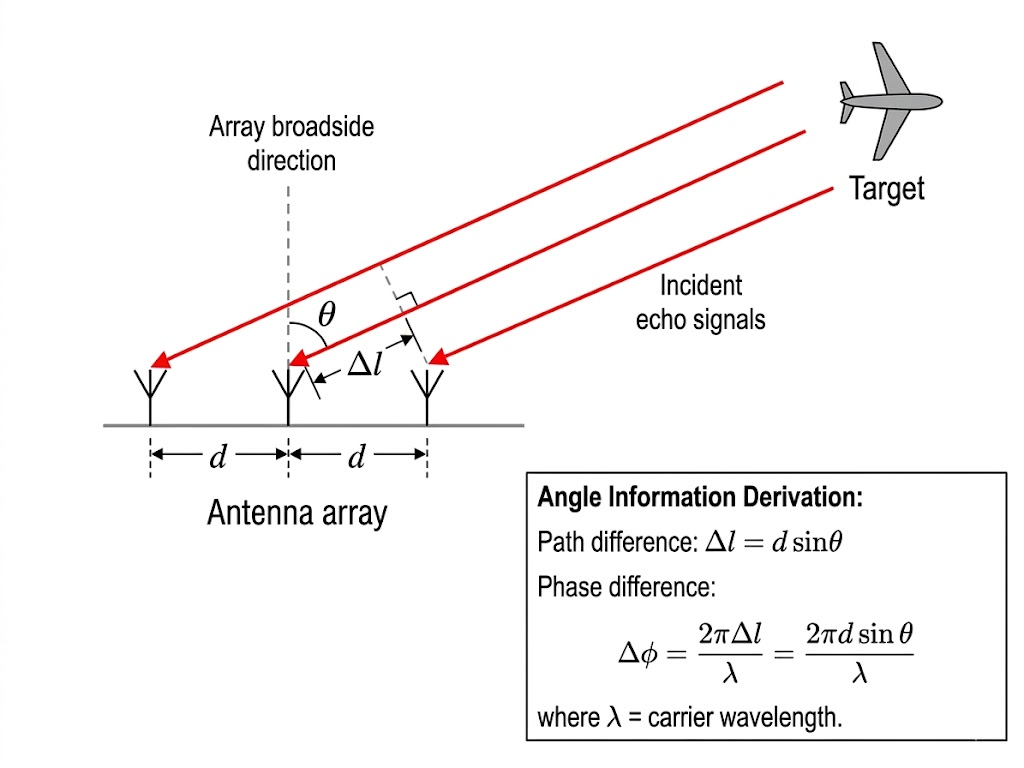
\includegraphics[width=0.62\textwidth]{figures/chapter2/fig_angle_estimation.jpeg}
    \caption{Angle estimation using an antenna array.}
    \label{fig:angle_estimation_antenna_array}
\end{figure}

The path difference further introduces a phase difference.
Since one wavelength \(\lambda\) corresponds to a phase change of \(2\pi\),
the phase difference corresponding to the path difference \(\Delta l\) is
\begin{equation}
    \Delta \phi = \frac{2\pi}{\lambda}\Delta l.
    \label{eq:path_phase_difference}
\end{equation}
Substituting \(\Delta l=d\sin\theta\) into the above expression gives the
phase difference between adjacent antenna elements as
\begin{equation}
    \Delta \phi = \frac{2\pi d\sin\theta}{\lambda}.
    \label{eq:array_phase_difference}
\end{equation}

Therefore, the target angle is encoded in the inter-element phase difference,
from which the direction of arrival can be inferred.

\subsection{Sensing Performance Metrics}

\topichead{Detection Performance}
Detection performance characterizes whether a sensing system can reliably
determine the presence or absence of a target under noise, clutter, and
interference.
It is commonly described by detection probability, false alarm probability,
and missed detection probability.

\topichead{Binary Hypothesis Model}
In radar sensing, target detection is commonly modeled as a binary hypothesis
testing problem.
Let \(\mathbf{y}\) be the received observation, \(\mathbf{s}\) the target echo
component, and \(\mathbf{n}\) the combined noise, clutter, and interference.
Then
\begin{equation}
    \begin{aligned}
        H_0 &: \quad \mathbf{y}=\mathbf{n}, \\
        H_1 &: \quad \mathbf{y}=\mathbf{s}+\mathbf{n}.
    \end{aligned}
    \label{eq:radar_binary_detection_model}
\end{equation}

Here, \(H_0\) represents the target-absent case and \(H_1\) represents the
target-present case.
The detector decides which hypothesis is more consistent with the observation
\(\mathbf{y}\).

\topichead{Detection Statistic and Threshold}
In practical detection, the receiver constructs a statistic \(T(\mathbf{y})\)
from the observation.
It may be the received energy, matched-filter output, correlation peak, a
range-Doppler cell magnitude, or a likelihood ratio.

After obtaining the detection statistic, the detector usually compares it with
a predefined threshold \(\gamma\) to make a binary decision:
\begin{equation}
    T(\mathbf{y})>\gamma \Rightarrow \text{decide } H_1,
    \label{eq:detection_decision_h1}
\end{equation}
\begin{equation}
    T(\mathbf{y})\leq\gamma \Rightarrow \text{decide } H_0.
    \label{eq:detection_decision_h0}
\end{equation}

The threshold \(\gamma\) therefore controls the detector decision and directly
affects detection probability and false alarm probability.

\topichead{Detection Outcomes and Probability Metrics}
Given the true state and the detector decision, four outcomes are possible, as
summarized in Table~\ref{tab:detection_outcomes}.

\begin{table}[htbp]
    \centering
    \caption{Basic outcomes of target detection.}
    \label{tab:detection_outcomes}
    \small
    \renewcommand{\arraystretch}{1.25}
    \begin{tabularx}{\textwidth}{
        >{\centering\arraybackslash}p{0.15\textwidth}
        >{\centering\arraybackslash}p{0.18\textwidth}
        >{\centering\arraybackslash}p{0.37\textwidth}
        >{\raggedright\arraybackslash}X
    }
        \toprule
        True target state
        & Detector decision
        & Conditional probability
        & Decision outcome \\
        \midrule

        \(H_0\)
        & Decide \(H_0\)
        & \(\Pr(\text{decide }H_0 \mid H_0)=1-P_{FA}\)
        & Correct no-target decision \\

        \(H_0\)
        & Decide \(H_1\)
        & \(P_{FA}=\Pr(\text{decide }H_1 \mid H_0)\)
        & False alarm \\

        \(H_1\)
        & Decide \(H_1\)
        & \(P_D=\Pr(\text{decide }H_1 \mid H_1)\)
        & Correct detection \\

        \(H_1\)
        & Decide \(H_0\)
        & \(P_M=\Pr(\text{decide }H_0 \mid H_1)=1-P_D\)
        & Missed detection \\
        \bottomrule
    \end{tabularx}
\end{table}

Here, \(P_{FA}\), \(P_D\), and \(P_M\) denote false alarm, detection, and missed
detection probabilities, respectively.
Since correct detection and missed detection are complementary under \(H_1\),
\begin{equation}
    P_D+P_M=1.
    \label{eq:detection_missed_relation}
\end{equation}
These probabilities characterize detector reliability from different
perspectives.

\topichead{Threshold Tradeoff}
Lowering \(\gamma\) generally increases the probability of deciding \(H_1\),
which may improve \(P_D\) but also increase \(P_{FA}\).
Raising \(\gamma\) suppresses false alarms but may miss weak targets.
Detector design therefore balances \(P_D\) and \(P_{FA}\), rather than
optimizing either metric in isolation.

\topichead{Neyman--Pearson Criterion}
The Neyman--Pearson criterion provides a classical rule for this tradeoff:
for a prescribed false alarm constraint \(P_{FA}=\alpha\), maximize the
detection probability \(P_D\).

Under this criterion, the classical decision rule is the likelihood-ratio test.
For the received observation \(\mathbf{y}\), the likelihood ratio is defined as
\begin{equation}
    \Lambda(\mathbf{y})
    =
    \frac{p(\mathbf{y}\mid H_1)}
         {p(\mathbf{y}\mid H_0)}.
    \label{eq:likelihood_ratio}
\end{equation}
The detector compares the likelihood ratio with a threshold \(\eta\):
\begin{equation}
    \Lambda(\mathbf{y})
    =
    \frac{p(\mathbf{y}\mid H_1)}
         {p(\mathbf{y}\mid H_0)}
    \mathop{\gtrless}_{H_0}^{H_1}
    \eta.
    \label{eq:np_likelihood_ratio_test}
\end{equation}
The threshold \(\eta\) is determined by the prescribed false alarm constraint,
namely,
\begin{equation}
    P_{FA}
    =
    P\left(\Lambda(\mathbf{y})>\eta\mid H_0\right)
    =
    \int_{\{\mathbf{y}:\Lambda(\mathbf{y})>\eta\}}
    p(\mathbf{y}\mid H_0)\,d\mathbf{y}
    =
    \alpha.
    \label{eq:np_false_alarm_constraint}
\end{equation}

Here, the likelihood ratio measures how strongly the observation supports
\(H_1\) relative to \(H_0\), and the threshold \(\eta\) is chosen to satisfy
the false alarm constraint.

As a simple illustration, consider a one-dimensional statistic \(T\):
\begin{equation}
    T\mid H_0 \sim \mathcal{N}(0,1),
    \qquad
    T\mid H_1 \sim \mathcal{N}(\mu,1).
    \label{eq:np_gaussian_statistic_model}
\end{equation}
where \(\mu>0\) is the mean shift caused by the target echo.
In this model, the likelihood-ratio test is equivalent to thresholding \(T\).

Given a false alarm constraint \(P_{FA}=\alpha\), the threshold \(\gamma\) is
determined by
\begin{equation}
    P(T>\gamma\mid H_0)=\alpha.
    \label{eq:np_threshold_from_pfa}
\end{equation}
Since \(T\mid H_0\sim\mathcal{N}(0,1)\), the threshold can be written as
\begin{equation}
    \gamma=\Phi^{-1}(1-\alpha),
    \label{eq:np_threshold_inverse_cdf}
\end{equation}
where \(\Phi^{-1}(\cdot)\) denotes the inverse cumulative distribution function
of the standard normal distribution.
Under the same threshold, the detection probability is given by
\begin{equation}
    P_D=P(T>\gamma\mid H_1).
    \label{eq:np_pd_from_threshold}
\end{equation}

Figure~\ref{fig:np_threshold_illustration} shows the two Gaussian densities and
the threshold \(\gamma\).
The false alarm probability is the area beyond \(\gamma\) under \(H_0\), while
the detection probability is the corresponding area under \(H_1\).

\begin{figure}[htbp]
    \centering
    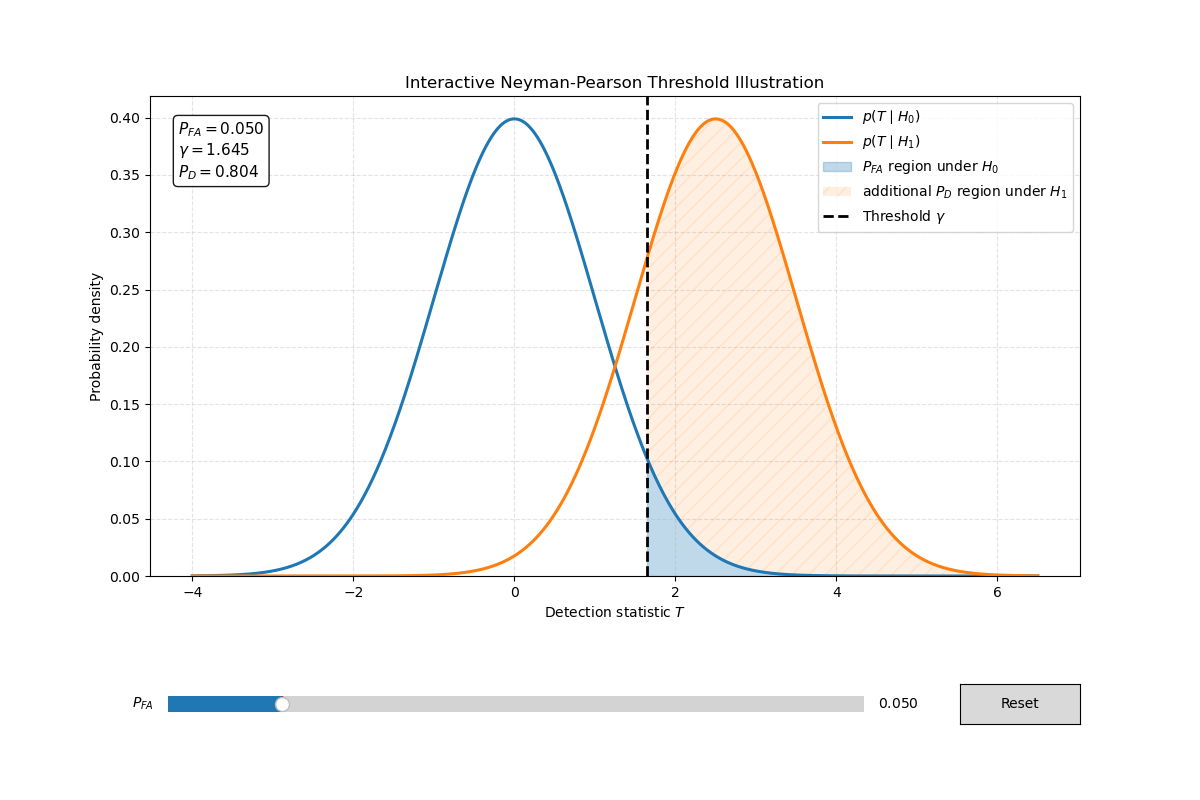
\includegraphics[width=0.66\textwidth]{figures/chapter2/fig_np_estimation.png}
    \caption{Illustration of Neyman--Pearson threshold selection using a one-dimensional Gaussian detection statistic.}
    \label{fig:np_threshold_illustration}
\end{figure}
The corresponding simulation script is listed in the Companion Code section.

\topichead{Resolution}
Resolution describes the ability to distinguish closely spaced targets in
range, velocity, or angle.
It is therefore a key metric for fine sensing capability.

Range resolution is based on resolving differences in echo delay.
Since the target range and the echo delay satisfy
\begin{equation}
    R=\frac{c\tau}{2},
    \label{eq:range_delay_resolution}
\end{equation}
the ability to resolve a smaller delay difference corresponds to the ability
to distinguish targets that are closer in range.
For a radar signal with bandwidth \(B\), the range resolution is commonly
approximated as
\begin{equation}
    \Delta R=\frac{c}{2B},
    \label{eq:range_resolution}
\end{equation}
where \(c\) is the propagation speed of the electromagnetic wave.
Thus, larger bandwidth improves range resolution.

As an example, consider a \(77\,\mathrm{GHz}\) millimeter-wave radar system.
If the signal bandwidth is \(B=1\,\mathrm{GHz}\), the range resolution is
approximately
\begin{equation}
    \Delta R
    =
    \frac{3\times 10^8}{2\times 1\times 10^9}
    =
    0.15\,\mathrm{m}.
    \label{eq:range_resolution_example}
\end{equation}
This gives an ideal range resolution of about \(0.15\,\mathrm{m}\).

Velocity resolution describes the ability to distinguish close radial
velocities and is mainly controlled by coherent observation time.
If the coherent observation time is denoted by \(T_{\mathrm{obs}}\), the
Doppler frequency resolution can be approximated as
\begin{equation}
    \Delta f_D \approx \frac{1}{T_{\mathrm{obs}}}.
    \label{eq:doppler_frequency_resolution}
\end{equation}
Combining this with the relationship between radial velocity and Doppler
frequency shift in a monostatic radar,
\begin{equation}
    v=\frac{\lambda f_D}{2},
    \label{eq:velocity_doppler_resolution}
\end{equation}
the velocity resolution can be approximated as
\begin{equation}
    \Delta v \approx \frac{\lambda}{2T_{\mathrm{obs}}},
    \label{eq:velocity_resolution}
\end{equation}
where \(\lambda\) is the carrier wavelength.
For a \(77\,\mathrm{GHz}\) radar, the carrier wavelength is approximately
\begin{equation}
    \lambda=\frac{c}{f_c}
    =
    \frac{3\times10^8}{77\times10^9}
    \approx 3.9\,\mathrm{mm}.
    \label{eq:wavelength_77ghz}
\end{equation}
If the coherent observation time is \(T_{\mathrm{obs}}=20\,\mathrm{ms}\), the
velocity resolution is approximately
\begin{equation}
    \Delta v
    \approx
    \frac{3.9\times10^{-3}}{2\times20\times10^{-3}}
    \approx
    0.098\,\mathrm{m/s}.
    \label{eq:velocity_resolution_example}
\end{equation}
For a fixed wavelength, a longer coherent observation time improves velocity
resolution.

Angle resolution describes the ability to distinguish close directions and is
mainly related to the effective antenna aperture.
For an array with effective aperture \(D\), the angle resolution is often
approximated as
\begin{equation}
    \Delta \theta \approx \frac{\lambda}{D},
    \label{eq:angle_resolution}
\end{equation}
where \(\lambda\) is the carrier wavelength and \(D\) denotes the effective
array aperture.

Again considering a \(77\,\mathrm{GHz}\) radar, if the effective array aperture
is \(D=4\,\mathrm{cm}\), the angle resolution is approximately
\begin{equation}
    \Delta \theta
    \approx
    \frac{3.9\times10^{-3}}{4\times10^{-2}}
    =
    0.0975\,\mathrm{rad}
    \approx
    5.6^\circ.
    \label{eq:angle_resolution_example}
\end{equation}
For a fixed wavelength, a larger aperture improves angle resolution, although
practical performance also depends on array geometry, beamforming, SNR, and
target location.

Table~\ref{tab:sensing_resolution_summary} summarizes the three resolution
metrics and the main physical factors that control them.
\begin{table}[htbp]
    \centering
    \caption{Compact summary of basic sensing resolution metrics.}
    \label{tab:sensing_resolution_summary}
    \small
    \renewcommand{\arraystretch}{1.25}
    \begin{tabularx}{\textwidth}{
        >{\raggedright\arraybackslash}p{0.17\textwidth}
        >{\raggedright\arraybackslash}p{0.21\textwidth}
        >{\centering\arraybackslash}p{0.18\textwidth}
        >{\raggedright\arraybackslash}p{0.18\textwidth}
        >{\raggedright\arraybackslash}X
    }
        \toprule
        Metric & Physical source & Approximate formula & Main controlling factor & Example implication \\
        \midrule
        Range resolution
        & Echo delay difference
        & \(\Delta R \approx c/(2B)\)
        & Signal bandwidth \(B\)
        & \(B=1\,\mathrm{GHz}\) gives \(\Delta R\approx0.15\,\mathrm{m}\). \\
        Velocity resolution
        & Doppler frequency difference
        & \(\Delta v \approx \lambda/(2T_{\mathrm{obs}})\)
        & Coherent observation time \(T_{\mathrm{obs}}\)
        & At \(77\,\mathrm{GHz}\), \(T_{\mathrm{obs}}=20\,\mathrm{ms}\) gives \(\Delta v\approx0.098\,\mathrm{m/s}\). \\
        Angle resolution
        & Array phase difference
        & \(\Delta\theta \approx \lambda/D\)
        & Effective aperture \(D\)
        & At \(77\,\mathrm{GHz}\), \(D=4\,\mathrm{cm}\) gives \(\Delta\theta\approx5.6^\circ\). \\
        \bottomrule
    \end{tabularx}
\end{table}

\topichead{Estimation Accuracy}
Estimation accuracy describes how close estimated target parameters are to
their true values.
It differs from resolution: resolution concerns whether nearby targets can be
separated, whereas accuracy concerns the correctness of the estimated range,
velocity, or angle of a detected target.

Let the true range, radial velocity, and angle of a target be denoted by
\(R\), \(v\), and \(\theta\), respectively.
Let the corresponding estimates be denoted by \(\hat{R}\), \(\hat{v}\), and
\(\hat{\theta}\).
The parameter estimation errors can then be defined as
\begin{equation}
    e_R=\hat{R}-R,\qquad
    e_v=\hat{v}-v,\qquad
    e_\theta=\hat{\theta}-\theta.
    \label{eq:parameter_estimation_errors}
\end{equation}
These errors measure deviations from the true parameters.
Statistical metrics such as mean squared error and root mean squared error are
commonly used:
For example, the mean squared error of range estimation can be written as
\begin{equation}
    \mathrm{MSE}_R
    =
    \mathbb{E}\left[(\hat{R}-R)^2\right],
    \label{eq:range_mse}
\end{equation}
and the corresponding root mean squared error is
\begin{equation}
    \mathrm{RMSE}_R
    =
    \sqrt{\mathbb{E}\left[(\hat{R}-R)^2\right]}.
    \label{eq:range_rmse}
\end{equation}
Similar metrics can be defined for velocity and angle.
Accuracy is affected by SNR, bandwidth, coherent observation time, array
aperture, target reflection, propagation environment, and estimation algorithm.
It directly influences tracking, localization, and beam pointing, so sensing
performance should consider not only detection and resolution but also
parameter-estimation accuracy.

\topichead{Sensing Coverage}
Sensing coverage describes the spatial or state region in which a system can
maintain reliable detection and parameter estimation.
It is a system-level metric covering range, angular, and velocity dimensions.
Range coverage is limited by echo power and round-trip propagation loss;
angular coverage depends on antenna pattern, array structure, and beam
scanning; and velocity coverage depends on the Doppler range that can be
observed and estimated without ambiguity.
Thus, coverage is not merely the geometric region a system can ``see'', but the
effective operating region under requirements on false alarm probability,
detection probability, and estimation error.
For ISAC, sensing coverage must also be considered together with communication
coverage, resource allocation, and beam scheduling.

\subsection{Radar Waveforms and Communication--Sensing Comparison}

\topichead{Typical Radar Waveforms and Processing Flow}
\topichead{Pulse Radar}
Pulse radar transmits a short pulse and receives the delayed echo reflected or
scattered by the target.
Because a more distant target produces a longer round-trip delay, range can be
estimated from the time difference between transmission and reception.

If the round-trip delay of the echo relative to the transmitted pulse is
denoted by \(\tau\), the target range can be expressed as
\[
    R=\frac{c\tau}{2},
\]
where \(c\) is the propagation speed of the electromagnetic wave.
The factor \(1/2\) comes from the two-way radar--target--radar propagation.
The basic concept is illustrated in Fig.~\ref{fig:pulse_radar_concept}.

\begin{figure}[htbp]
    \centering
    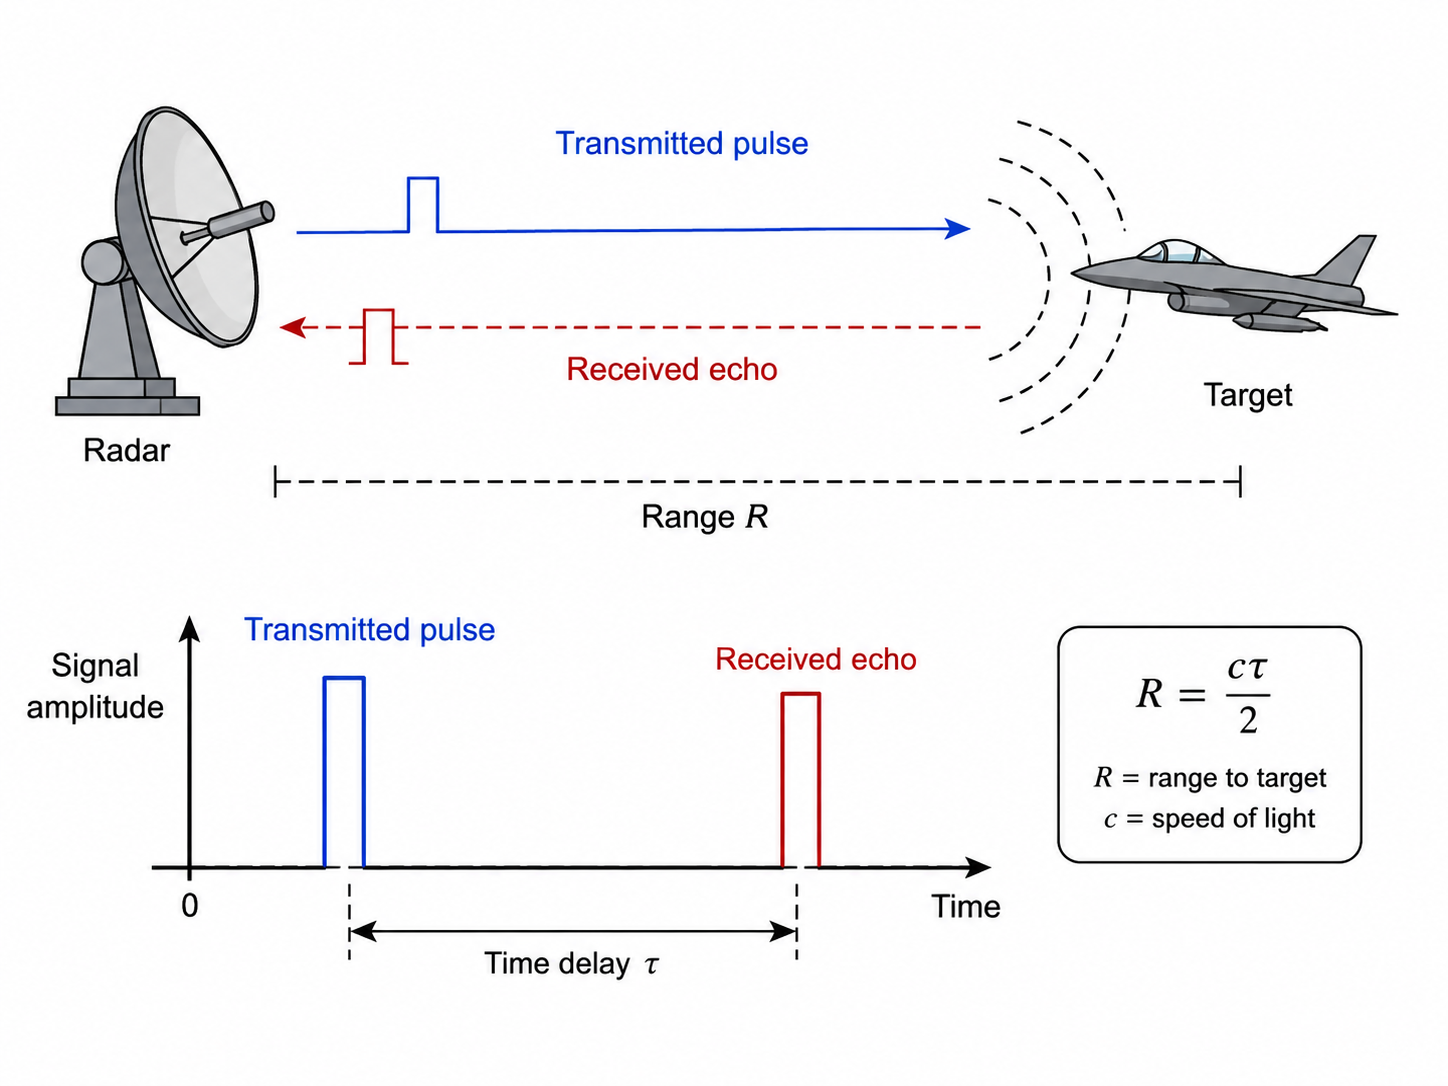
\includegraphics[width=0.62\textwidth]{figures/chapter2/fig_pulse_radar.png}
    \caption{Concept of pulse radar.}
    \label{fig:pulse_radar_concept}
\end{figure}

Pulse radar provides direct ranging intuition, but pulse width, bandwidth,
transmitted energy, and range resolution are coupled.
Practical systems often use modulated pulses with pulse compression or matched
filtering to balance detection capability and range resolution.

\topichead{Continuous-Wave Radar}
Continuous-wave radar transmits a continuous single-frequency or approximately
single-frequency signal.
A stationary target returns an echo with approximately the same frequency,
whereas radial motion produces a Doppler shift.
Thus, continuous-wave radar is mainly used for velocity sensing, as illustrated
in Fig.~\ref{fig:cw_radar_concept}.

\begin{figure}[htbp]
    \centering
    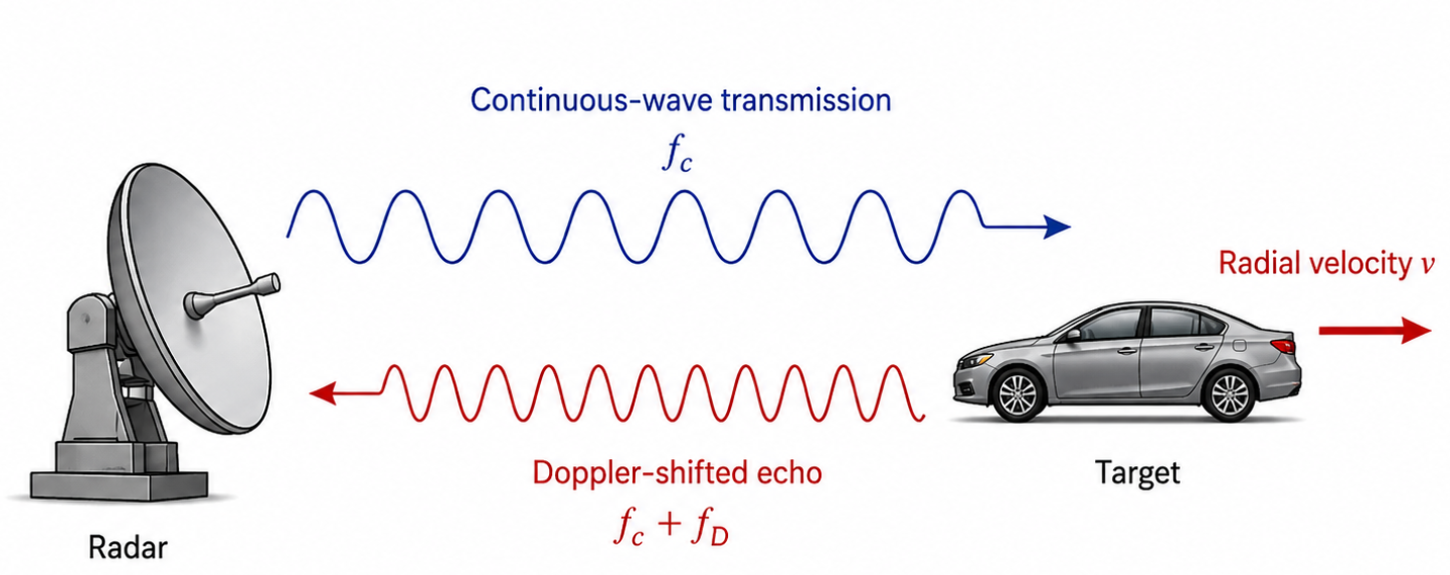
\includegraphics[width=0.64\textwidth]{figures/chapter2/fig_cw_radar.png}
    \caption{Concept of continuous-wave radar.}
    \label{fig:cw_radar_concept}
\end{figure}

As introduced earlier, for a monostatic radar, the Doppler frequency shift is
related to the radial velocity by
\[
    f_D=\frac{2v}{\lambda},
    \qquad
    v=\frac{\lambda f_D}{2}.
\]
Here, \(\lambda\) denotes the carrier wavelength.

Because a pure single-frequency continuous wave has no explicit time marker,
its direct ranging capability is limited.
Varying the transmitted frequency with time converts delay into a measurable
frequency difference, leading to FMCW radar.

\topichead{Frequency-Modulated Continuous-Wave Radar}
Frequency-modulated continuous-wave radar transmits a continuous signal whose
frequency varies with time.
For a linear chirp,
\[
    f(t)=f_0+St,
\]
where \(f_0\) is the starting frequency and \(S\) is the chirp slope.
If the echo has delay \(\tau\), mixing it with the local transmitted signal
produces a beat frequency \(f_b\).
Figure~\ref{fig:fmcw_chirp_sequence} illustrates a simplified
\(77\,\mathrm{GHz}\) chirp sequence.

\begin{figure}[htbp]
    \centering
    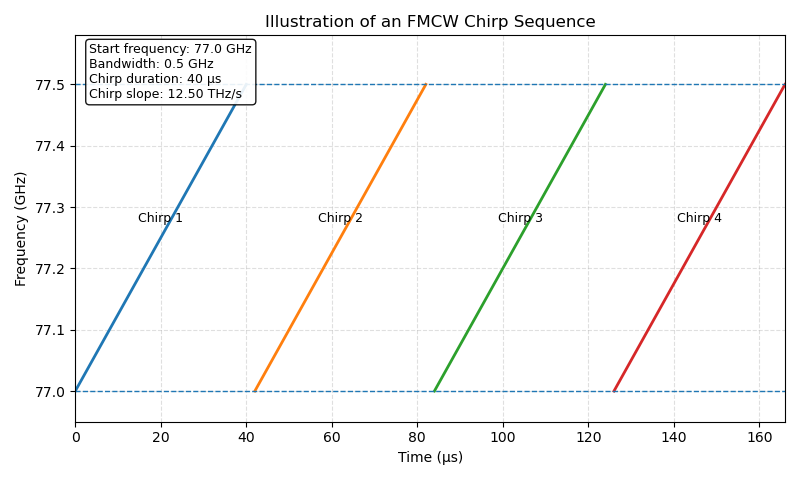
\includegraphics[width=0.66\textwidth]{figures/chapter2/fig_fmcw_chirp_sequence.png}
    \caption{Illustration of an FMCW chirp sequence in the \(77\,\mathrm{GHz}\) band.}
    \label{fig:fmcw_chirp_sequence}
\end{figure}

For a linear chirp, ignoring Doppler or assuming low target velocity gives
\[
    f_b \approx S\tau.
\]
Combining this relationship with the delay--range relation
\[
    R=\frac{c\tau}{2},
\]
the target range can be approximated as
\[
    R\approx \frac{c f_b}{2S}.
\]

FMCW radar therefore maps propagation delay into a measurable frequency
difference.
For a fixed chirp slope, a larger range produces a larger beat frequency.
Figure~\ref{fig:fmcw_beat_frequency} illustrates this beat-frequency formation
for a representative target range.

\begin{figure}[htbp]
    \centering
    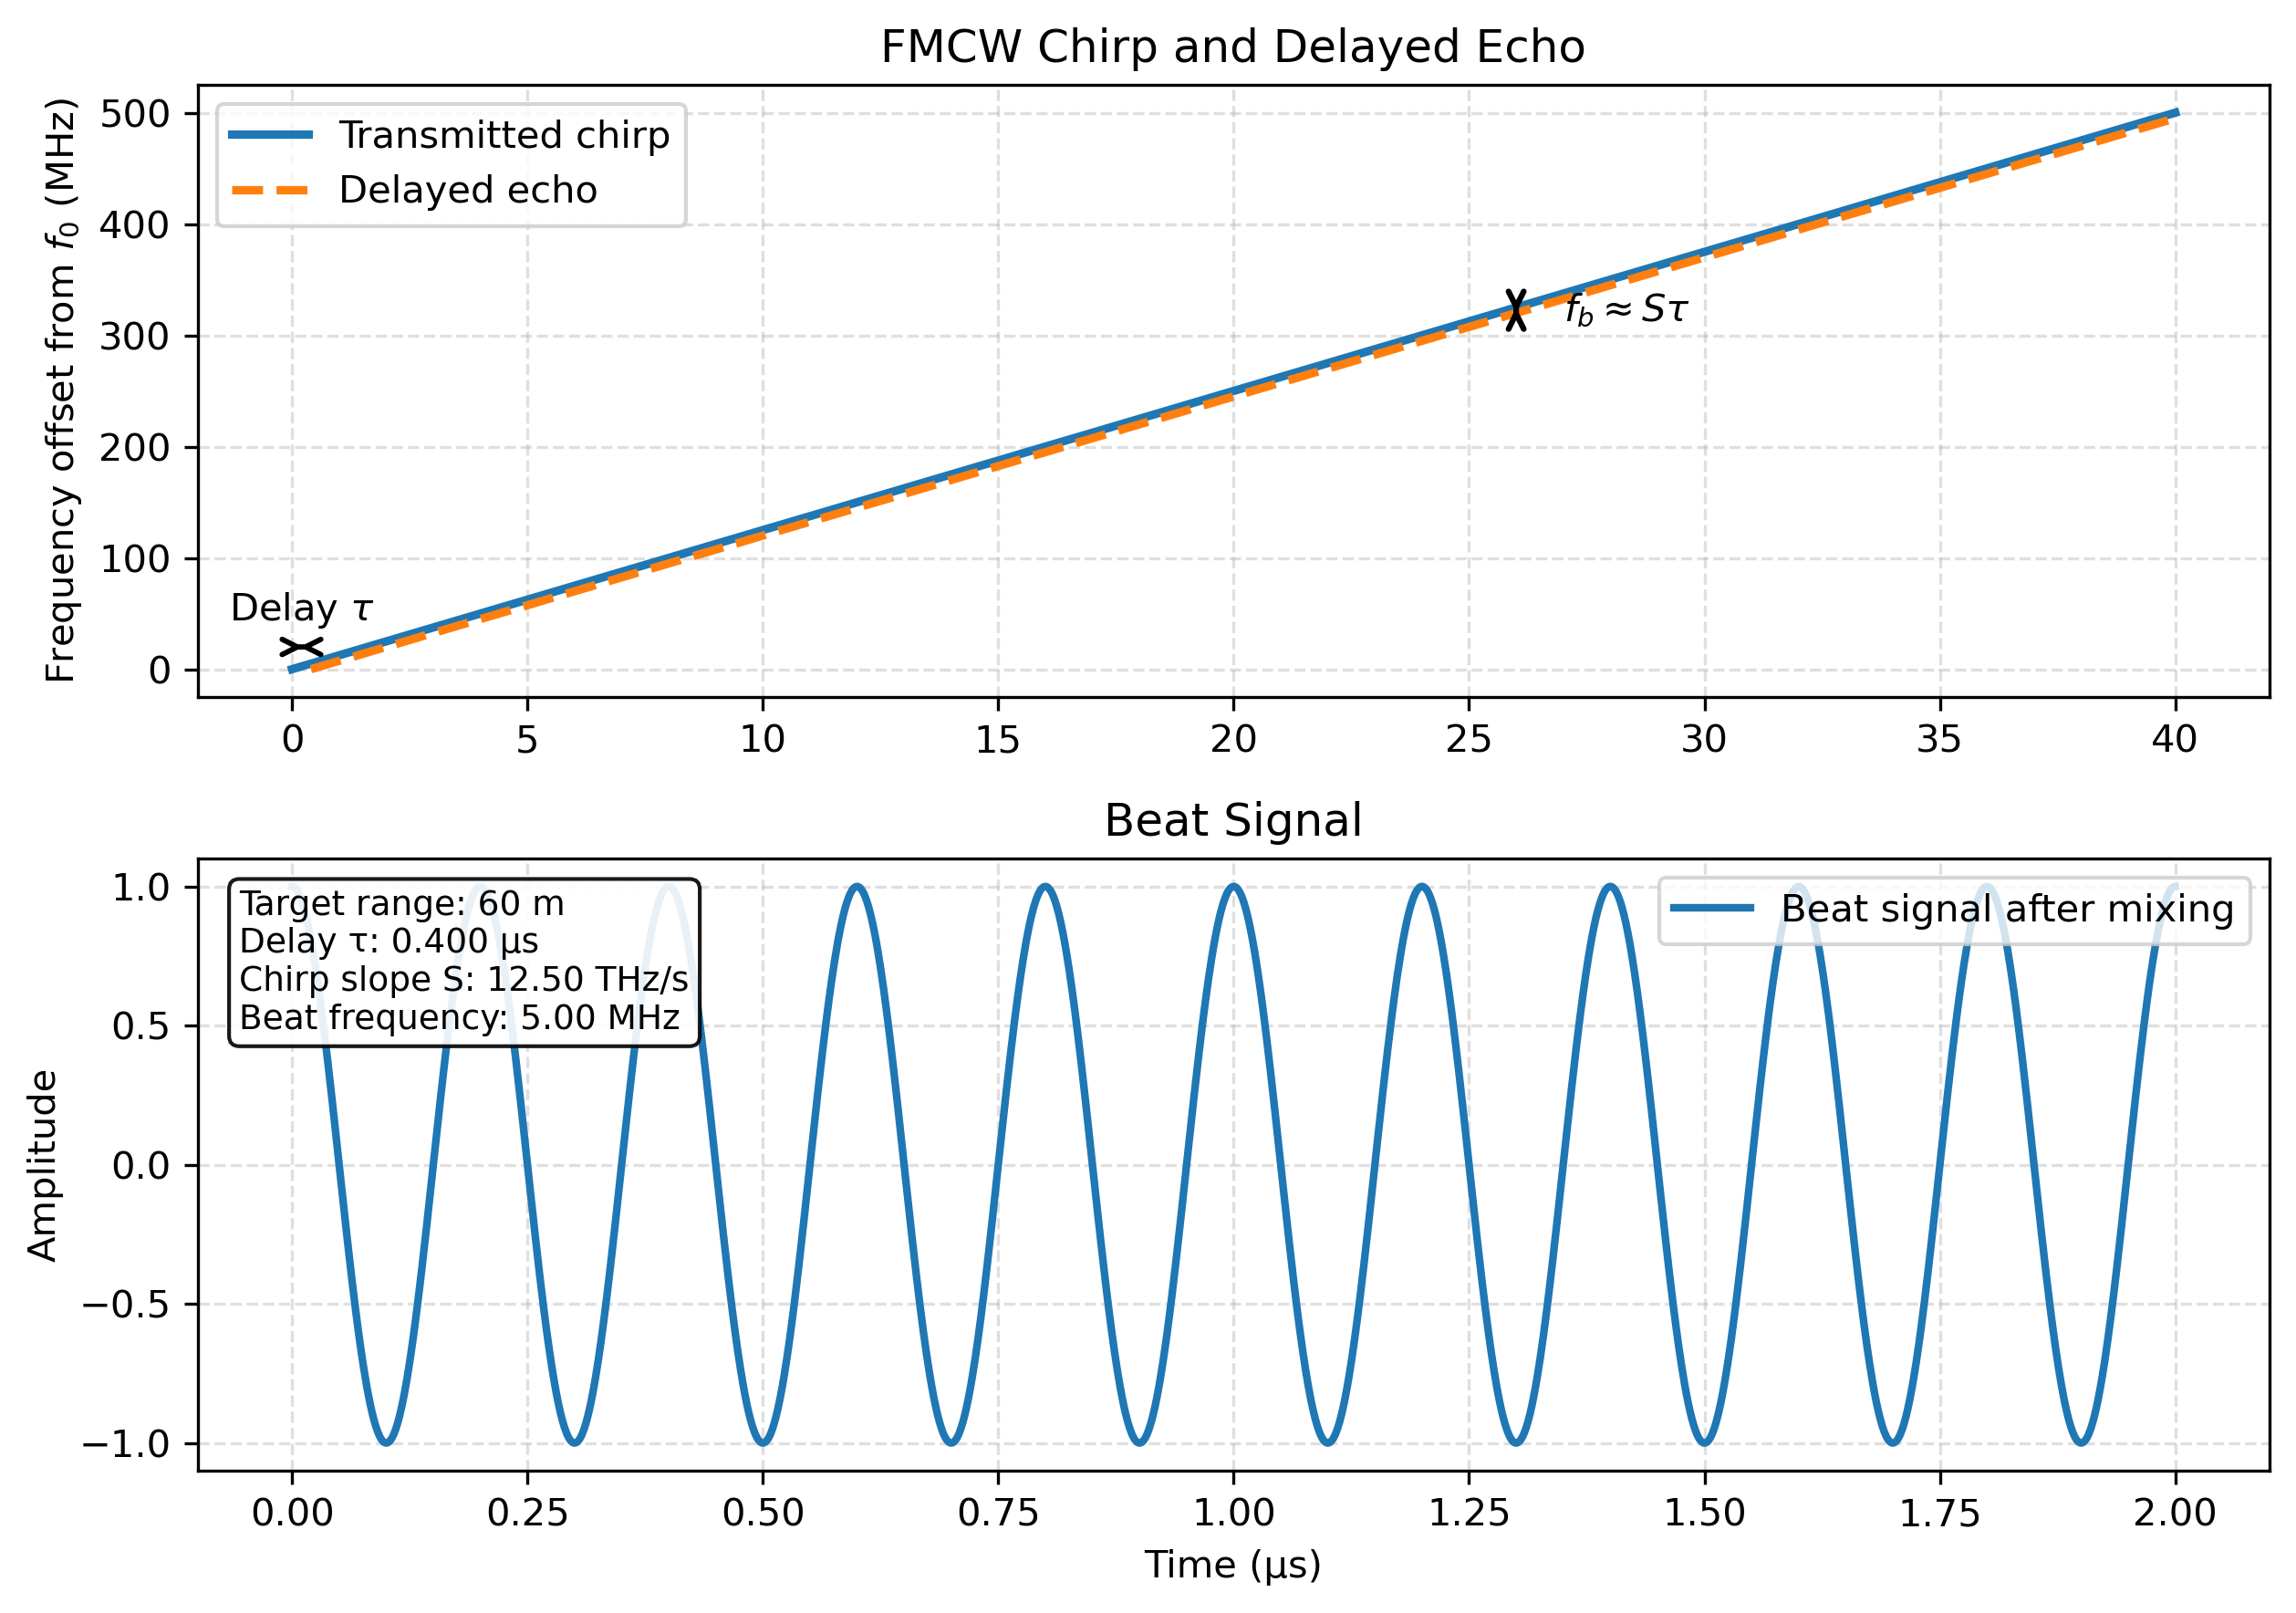
\includegraphics[width=0.66\textwidth]{figures/chapter2/fig_fmcw_beat_frequency.png}
    \caption{Illustration of beat frequency formation in FMCW radar.}
    \label{fig:fmcw_beat_frequency}
\end{figure}

The corresponding simulation scripts are listed in the Companion Code section.
When radial motion is significant, Doppler also affects the beat frequency.
Practical FMCW systems usually transmit multiple chirps: fast-time samples are
used for range processing, while slow-time variation across chirps supports
Doppler and velocity estimation.

\topichead{Comparison Between Digital Communication and Radar Sensing}

\topichead{Common Characteristics}
Digital communication and radar sensing are designed for different tasks, but
both rely on wireless electromagnetic propagation and signal processing.
In both systems, a designed signal is transmitted, propagates through the
environment, is observed at the receiver, and is processed to extract useful
information.
They therefore share foundations in propagation, hardware architecture,
synchronization, array processing, interference handling, and receiver design.

\topichead{Fundamental Differences}
The main difference lies in objectives and interpretation of the received
signal.
Communication aims to recover information bits or symbols reliably in the
presence of channel effects, noise, and interference.
Radar sensing aims to infer environmental information from echoes, including
target existence, range, velocity, angle, and reflection properties.
Thus, the wireless channel is mainly a medium to be compensated in
communication, whereas in sensing the propagation response itself carries the
desired physical information.
The propagation path also differs: communication links are usually one-way,
whereas monostatic radar echoes experience two-way propagation and target
reflection, leading to stronger distance-dependent attenuation.

\topichead{Basis for Integration}
The basis for integration is also clear.
Both functions use the same propagation medium and scarce spectrum resources,
and modern communication systems already employ wideband radio-frequency
front ends, large antenna arrays, beamforming, and high-speed digital signal
processing.
Many tools, including synchronization, correlation, frequency-domain analysis,
array processing, detection, and estimation, are useful for both communication
and sensing.

\topichead{Challenges of Integration}
Integration is nevertheless challenging.
Communication metrics such as BER, throughput, spectral efficiency, latency,
and reliability differ from sensing metrics such as detection probability,
false alarm probability, resolution, estimation accuracy, and coverage.
Preferred waveforms and receiver processing flows also differ: communication
emphasizes information recovery and multi-user transmission, whereas sensing
emphasizes echo enhancement, parameter estimation, and tracking.
ISAC therefore requires joint design across waveform design, hardware
architecture, resource allocation, and receiver processing.
The common foundations make integration possible, while the differences
determine the complexity of ISAC system design.